\documentclass[a4paper,12pt]{article}
\usepackage[utf8]{vietnam}
\usepackage{hyperref}
\usepackage{graphicx}
\usepackage{xcolor}
\usepackage{subfigure}
\usepackage{float}
\usepackage{caption}
\usepackage{placeins}
\makeatletter
\setlength{\@fptop}{0pt}
\makeatother
\hypersetup{
	pdfborder = {0 0 0}
}
\title{\textbf{Báo cáo tuần 11(2) \\ Thực hành kiến trúc máy tính}}
\author{Họ tên: Phan Minh Anh Tuấn \\ MSSV: 20205227}
\date{}
\begin{document}
	\maketitle
	\tableofcontents
	\newpage
	\section{Assignment 4}
	Chương trình thực hiện ngắt khi có phím nào đó được bấm hoặc khi hết một khoảng thời gian. Mỗi khi có phím được bấm, chương trình sẽ in mã của phím đó cùng số lần ngắt theo thời gian giữa 2 lần bấm phím ra màn hình. \\
	Mã của các phím như sau:
	\FloatBarrier
	\begin{figure}[ht!]
		\centerline{\fbox{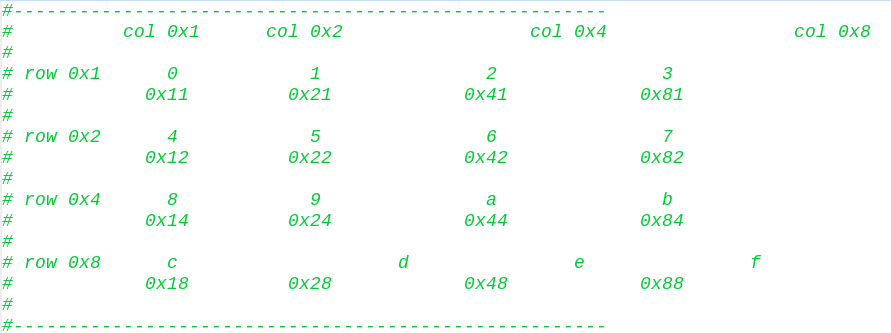
\includegraphics[width=1\textwidth]{ass4/ma.png}}}
		\caption{Mã của các phím}
		\label{fig:ass1}
	\end{figure}
	\noindent
Chương trình con thực hiện ngắt nằm ở địa chỉ cố định 0x80000180. Khi có một phím được bấm, chương trình chính sẽ ngắt vì ta đã nạp giá trị vào địa chỉ IN\_ADDRESS\_HEXA\_KEYBOARRD là 0x80, bit số 7 bằng 1 để cho phép ngắt:
\FloatBarrier
\begin{figure}[ht!]
	\centerline{\fbox{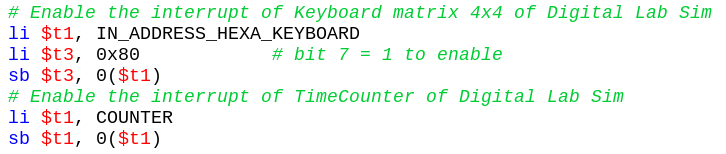
\includegraphics[width=1\textwidth]{ass4/a.png}}}
	\caption*{}
	\label{fig:ass1}
\end{figure}
\clearpage
\noindent
Chương trình cũng ngắt sau mỗi khoảng thời gian nhất định vì ta bật ngắt theo thời gian của Digital Lab Sim:
\FloatBarrier
\begin{figure}[ht!]
	\centerline{\fbox{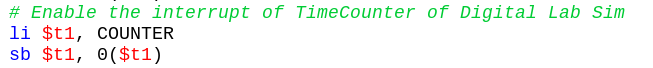
\includegraphics[width=1\textwidth]{ass4/b.png}}}
	\caption*{}
	\label{fig:ass1}
\end{figure}
\noindent
Sau đó ta gán biến đếm số lần ngắt theo thời gian bằng 0:
\end{document}